% SOURCE: Chinese PDF viewer pp. 144 (lower part)--151 (upper part).
% Source p. 146 contains only the completion of the question on p. 145;
% source p. 147 restarts the original pagination without starting a new chapter.
\section{Exchange Symmetry of Identical Particles}
\textbf{Identical particles:} Particles whose intrinsic properties (mass, charge, spin, etc.) are completely identical.

In classical mechanics, because physical quantities are continuous, the properties of two particles may be arbitrarily close, but cannot be completely identical, and the particles can always be distinguished. Hence the concept of identical particles does not arise in classical mechanics. In quantum mechanics, the values of physical quantities can be discrete, so particles may be completely identical or completely different. Thus the problem of identical particles arises.

How should identical particles be distinguished?

\subsection*{1) Principle of indistinguishability}
Even in classical mechanics there are ``identical'' particles; one may nevertheless distinguish them by their trajectories. In quantum mechanics there are no trajectories, and states are described by wavefunctions. Consider two noninteracting identical particles, with single-particle states $\psi_n(x)$ and $\psi_m(x)$. When their wavefunctions do not overlap, the two identical particles can be distinguished. When the wavefunctions overlap, if one finds a particle in the overlap region, one cannot distinguish whether it is the first or the second particle; thus identical particles become indistinguishable where the wavefunctions overlap.

\begin{center}
\begin{tikzpicture}[x=1.0cm,y=0.9cm,>=Latex]
  \draw (-.25,0)--(4.35,0);
  \draw[thick,domain=0.25:1.75,samples=50] plot (\x,{1.15*exp(-7*(\x-1)^2)});
  \draw[thick,domain=2.45:3.95,samples=50] plot (\x,{1.15*exp(-7*(\x-3.2)^2)});
  \node at (1.0,1.45) {$\psi_n(x_1)$};
  \node at (3.2,1.45) {$\psi_m(x_2)$};
  \begin{scope}[xshift=6.1cm]
  \draw (-.25,0)--(4.35,0);
  \draw[thick,domain=0.25:2.75,samples=50] plot (\x,{1.15*exp(-2.6*(\x-1.3)^2)});
  \draw[thick,domain=1.55:4.05,samples=50] plot (\x,{1.15*exp(-2.6*(\x-3.0)^2)});
  \fill[pattern=north east lines,pattern color=gray!70] (1.65,0)--plot[domain=1.65:2.14,samples=24] (\x,{1.15*exp(-2.6*(\x-1.3)^2)})--plot[domain=2.14:1.65,samples=24] (\x,{1.15*exp(-2.6*(\x-3.0)^2)})--cycle;
  \node at (1.2,1.5) {$\psi_n(x_1)$};
  \node at (3.15,1.5) {$\psi_m(x_2)$};
  \end{scope}
\end{tikzpicture}
\end{center}

Strictly speaking, wavefunctions overlap throughout space. Thus, when the positions of two particles are exchanged, i.e., when
\[\{\psi_n(x_1),\psi_m(x_2)\}
\longrightarrow\{\psi_n(x_2),\psi_m(x_1)\},\]
the observed probability distribution is the same and the state is unchanged. The states described by the two sets of wavefunctions are the same state of the identical-particle system.

\textbf{Principle of indistinguishability:} Exchanging two identical particles does not change the state of the system.

\textbf{Question.} What restrictions does this principle impose on the state?

\subsection*{2) Exchange symmetry of wavefunctions}
For a system of $N$ identical particles, let its state be $\ket{i\ldots j\ldots}$ and define the exchange operator $\op P_{ij}$:
\[\op P_{ij}\ket{i\ldots j\ldots}
=\ket{j\ldots i\ldots}
=\lambda\ket{i\ldots j\ldots}.\]
The second equality uses the principle of indistinguishability. Since
\[\op P_{ij}^{\,2}\ket{i\ldots j\ldots}
=\op P_{ij}\ket{j\ldots i\ldots}
=\ket{i\ldots j\ldots},\]
the eigenvalues of $\op P_{ij}^{\,2}$ are $1$, and the eigenvalues of $\op P_{ij}$ are $\lambda=\pm1$. Hence
\[\op P_{ij}\ket{i\ldots j\ldots}
=\pm\ket{i\ldots j\ldots}.\]

\textbf{Exchange symmetry:} Under exchange of any two particles, the wavefunction of an identical-particle system must be either symmetric or antisymmetric.

\textbf{Question.} Can the wavefunction of an identical-particle system be symmetric at one time and antisymmetric at another?

If the Hamiltonian $\op H$ of the identical-particle system has exchange symmetry,
\[\op P_{ij}\op H\op P_{ij}^{-1}=\op H,\qquad
[\op P_{ij},\op H]=0,\]
then $\op P_{ij}$ is conserved. If the system is initially in a particular eigenstate of $\op P_{ij}$ (a symmetric or antisymmetric state), it remains in that eigenstate. Thus the wavefunction's exchange symmetry does not vary with time.

Experiments show that exchange symmetry is determined by spin. For an identical-particle system consisting of bosons (particles with integer spin), the state is symmetric under exchange. For a system of fermions (particles with half-integer spin), the state is antisymmetric under exchange.

\textbf{Question.} The state of an identical-particle system must satisfy exchange symmetry and the Schr\"odinger equation. How can states satisfying both requirements be constructed?

\subsection*{3) States of two identical particles}
Suppose
\[\op H(1,2)\psi(1,2)=E\psi(1,2).\]
Act on both sides with the exchange operator $\op P_{12}$:
\[\op P_{12}\op H(1,2)\op P_{12}^{-1}\op P_{12}\psi(1,2)
=E\op P_{12}\psi(1,2).\]
Since the Hamiltonian has exchange symmetry,
\[\op H(1,2)=\op H(2,1),\]
we have
\[\op H(1,2)\psi(2,1)=E\psi(2,1).\]
Thus $\psi(1,2)$ and $\psi(2,1)$ are eigenstates of $\op H$ belonging to the same eigenvalue $E$.

If $\psi(1,2)$ does not satisfy exchange symmetry, i.e., $\psi(2,1)\ne\pm\psi(1,2)$, one can construct symmetric or antisymmetric wavefunctions:
\begin{align*}
\text{Boson system:}\qquad&\psi_+(1,2)=\psi(1,2)+\psi(2,1),\\
\text{Fermion system:}\qquad&\psi_-(1,2)=\psi(1,2)-\psi(2,1).
\end{align*}
They remain eigenstates of $\op H$ with eigenvalue $E$:
\[\op H\psi_\pm(1,2)=E\psi_\pm(1,2).\]

\textbf{Example.} If interactions between particles are neglected,
\[\op H(1,2)=\op H_0(1)+\op H_0(2),\]
solve
\[\op H\psi(1,2)=E\psi(1,2).\]
Let
\[\op H_0\varphi_n(i)=\varepsilon_n\varphi_n(i),\qquad i=1,2.\]
Then
\[E=\varepsilon_n+\varepsilon_m,\qquad
\psi(1,2)=\varphi_n(1)\varphi_m(2).\]
In general, $\psi(1,2)$ does not satisfy exchange symmetry. To meet the requirement, the boson system has
\[
\psi_+(1,2)=\begin{cases}
\dfrac1{\sqrt2}[\varphi_n(1)\varphi_m(2)+\varphi_n(2)\varphi_m(1)],&n\ne m,\\[5pt]
\varphi_n(1)\varphi_n(2),&n=m.
\end{cases}
\]
For the fermion system,
\[\psi_-(1,2)=\frac1{\sqrt2}
[\varphi_n(1)\varphi_m(2)-\varphi_n(2)\varphi_m(1)]
=\frac1{\sqrt2}\begin{vmatrix}
\varphi_n(1)&\varphi_n(2)\\
\varphi_m(1)&\varphi_m(2)
\end{vmatrix}.\]
For fermions, if both particles occupy the same state (with the same quantum numbers), $n=m$ and $\psi_-(1,2)=0$. Hence:

\textbf{Pauli exclusion principle:} Two identical fermions cannot occupy the same state.

It should be emphasized that, before exchange symmetrization, the many-particle wavefunction assigns individual particles to particular single-particle states. After exchange symmetrization, it specifies how many particles occupy each single-particle state, and no longer specifies each particle's state.

The above discussion of wavefunction exchange symmetry extends to many identical-particle systems, leading to second quantization and quantum field theory.

\subsection*{4) Observable effects of identical particles}
\textbf{Example 1: Spatial wavefunctions of two free particles.}

\textbf{a) Without taking identity into account.}
\[\psi(\vect r_1,\vect r_2)=\frac1{(2\pi\hbar)^3}
 e^{\ii(\vect k_1\cdot\vect r_1+\vect k_2\cdot\vect r_2)}.\]
Introduce the center-of-mass and relative coordinates,
\[\vect R=\frac12(\vect r_1+\vect r_2),\qquad
\vect r=\vect r_1-\vect r_2,\]
the total and relative wavevectors,
\[\vect K=\vect k_1+\vect k_2,\qquad
\vect k=\frac12(\vect k_1-\vect k_2).\]
The wavefunction is
\[\psi(\vect R,\vect r)=\frac1{(2\pi\hbar)^3}
 e^{\ii\vect K\cdot\vect R}e^{\ii\vect k\cdot\vect r}.\]
Taking one particle as the center, the probability of finding the other particle inside a spherical shell of radius $r$ and thickness $\dd r$ is
\[P(r)=\int|\psi(\vect R,\vect r)|^2\,\dd^3R\,r^2\dd\Omega
=Ar^2.\]

\textbf{b) Two identical bosons.}
\[\psi_+(\vect r_1,\vect r_2)=\frac1{\sqrt2}
[\psi(\vect r_1,\vect r_2)+\psi(\vect r_2,\vect r_1)],\]
\begin{align*}
\psi_+(\vect R,\vect r)
&=\frac{e^{\ii\vect K\cdot\vect R}}{(2\pi\hbar)^3}
\frac1{\sqrt2}\left(e^{\ii\vect k\cdot\vect r}+e^{-\ii\vect k\cdot\vect r}\right)\\
&=\frac{\sqrt2}{(2\pi\hbar)^3}
\cos(\vect k\cdot\vect r)e^{\ii\vect K\cdot\vect R}.
\end{align*}
The probability is
\[P_+(r)=\int|\psi_+(\vect R,\vect r)|^2\,
\dd^3R\,r^2\dd\Omega
=Ar^2\left(1+\frac{\sin(2kr)}{2kr}\right).\]

\textbf{c) Antisymmetric wavefunction.}
\[\psi_-(\vect r_1,\vect r_2)=\frac1{\sqrt2}
[\psi(\vect r_1,\vect r_2)-\psi(\vect r_2,\vect r_1)],\]
\[\psi_-(\vect R,\vect r)=\frac{\sqrt2\ii}{(2\pi\hbar)^3}
\sin(\vect k\cdot\vect r)e^{\ii\vect K\cdot\vect R},\]
\[P_-(r)=Ar^2\left(1-\frac{\sin(2kr)}{2kr}\right).\]

\begin{center}
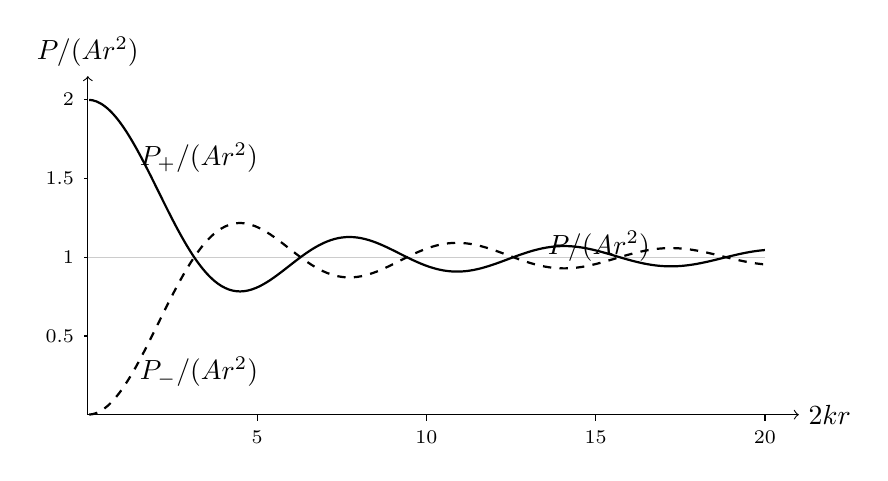
\begin{tikzpicture}[x=0.43cm,y=2.0cm]
\draw[->] (0,0)--(21,0) node[right] {$2kr$};
\draw[->] (0,0)--(0,2.15) node[above] {$P/(Ar^2)$};
\draw[gray!40] (0,1)--(20,1);
\foreach \x in {5,10,15,20}{\draw (\x,0)--(\x,-.04) node[below,font=\scriptsize]{\x};}
\foreach \y in {0.5,1,1.5,2}{\draw (0,\y)--(-.12,\y) node[left,font=\scriptsize]{\y};}
\draw[thick,domain=0.04:20,samples=180,smooth] plot (\x,{1+sin(\x r)/\x});
\draw[thick,dashed,domain=0.04:20,samples=180,smooth] plot (\x,{1-sin(\x r)/\x});
\node[anchor=west] at (1.25,1.63) {$P_+/(Ar^2)$};
\node[anchor=west] at (1.25,.27) {$P_-/(Ar^2)$};
\node[anchor=west] at (13.3,1.07) {$P/(Ar^2)$};
\end{tikzpicture}
\end{center}

This shows that a symmetric spatial wavefunction increases the probability of finding two particles close together, whereas an antisymmetric spatial wavefunction decreases that probability. There seems to be a kind of force between identical particles: bosons seem to attract and fermions to repel. This is called an \emph{exchange force}. It is not a force in the genuine sense; it has no agent exerting it, and it disappears at $r\to\infty$.

\textbf{Example 2: Expectation value of a mechanical quantity for a two-particle system.}

Let the mechanical quantity be $\op F(|\vect r_1-\vect r_2|)$. Without considering exchange symmetry,
\[\langle F\rangle=\int\psi^*(\vect r_1,\vect r_2)
\op F(|\vect r_1-\vect r_2|)\psi(\vect r_1,\vect r_2)
\,\dd^3r_1\dd^3r_2.\]
Taking exchange symmetry into account,
\begin{align*}
\langle F\rangle_\pm
&=\int\psi_\pm^*(\vect r_1,\vect r_2)
\op F(|\vect r_1-\vect r_2|)\psi_\pm(\vect r_1,\vect r_2)
\,\dd^3r_1\dd^3r_2\\
&=\int\frac1{\sqrt2}[\psi^*(\vect r_1,\vect r_2)\pm\psi^*(\vect r_2,\vect r_1)]
\op F(|\vect r_1-\vect r_2|)
\frac1{\sqrt2}[\psi(\vect r_1,\vect r_2)\pm\psi(\vect r_2,\vect r_1)]
\,\dd^3r_1\dd^3r_2\\
&=\frac12\int\Bigl[
\psi^*(\vect r_1,\vect r_2)\op F\psi(\vect r_1,\vect r_2)
+\psi^*(\vect r_2,\vect r_1)\op F\psi(\vect r_2,\vect r_1)\\
&\hspace{36mm}\pm\psi^*(\vect r_1,\vect r_2)\op F\psi(\vect r_2,\vect r_1)
\pm\psi^*(\vect r_2,\vect r_1)\op F\psi(\vect r_1,\vect r_2)
\Bigr]\,\dd^3r_1\dd^3r_2\\
&=\langle F\rangle\pm
\int\psi^*(\vect r_1,\vect r_2)
\op F(|\vect r_1-\vect r_2|)
\psi(\vect r_2,\vect r_1)\,\dd^3r_1\dd^3r_2\\
&\ne\langle F\rangle.
\end{align*}

\subsection*{5) Spin wavefunctions of two identical fermions}
The total wavefunction is
\[\psi(\vect r_1,s_{1z};\vect r_2,s_{2z}).\]
If coupling between configuration space and spin space is neglected, i.e., $\op{\vect L}\cdot\op{\vect S}$ coupling, then
\[\psi(\vect r_1,s_{1z};\vect r_2,s_{2z})
=\psi(\vect r_1,\vect r_2)\chi(s_{1z},s_{2z}).\]
(The total Hilbert space is the direct product of configuration space and spin space.)

The requirement of antisymmetry of the total wavefunction under exchange is:
\begin{enumerate}[label=\alph*)]
\item symmetric spatial wavefunction $\psi_+(\vect r_1,\vect r_2)$ and\\ antisymmetric spin wavefunction $\chi_-(s_{1z},s_{2z})$;
\item antisymmetric spatial wavefunction $\psi_-(\vect r_1,\vect r_2)$ and\\ symmetric spin wavefunction $\chi_+(s_{1z},s_{2z})$.
\end{enumerate}
If coupling between $\op{\vect s}_1$ and $\op{\vect s}_2$ is further neglected, the total spin wavefunction is a direct product of eigenstates of the single-fermion spin operator $\op s_z$:
\[\chi(s_{1z},s_{2z})=\chi(s_{1z})\chi(s_{2z})
=\begin{cases}
\chi_+(1)\chi_+(2),\\
\chi_+(1)\chi_-(2),\\
\chi_-(1)\chi_+(2),\\
\chi_-(1)\chi_-(2).
\end{cases}\]
Four independent symmetric or antisymmetric spin states can be constructed:
\begin{align*}
\chi_+^1(s_{1z},s_{2z})&=\chi_+(1)\chi_+(2),\\
\chi_+^2(s_{1z},s_{2z})&=\frac1{\sqrt2}
[\chi_+(1)\chi_-(2)+\chi_+(2)\chi_-(1)],\\
\chi_+^3(s_{1z},s_{2z})&=\chi_-(1)\chi_-(2),\\
\chi_-(s_{1z},s_{2z})&=\frac1{\sqrt2}
[\chi_+(1)\chi_-(2)-\chi_+(2)\chi_-(1)].
\end{align*}
It is easy to prove that they are eigenstates of the total spin operators
\[\op{\vect S}^{\,2}=(\op{\vect s}_1+\op{\vect s}_2)^2,
\qquad\op S_z=\op s_{1z}+\op s_{2z}.\]
Their eigenvalues and eigenstates are:
\[
\begin{array}{c|c|c}
\text{Eigenstate}&\text{Total spin}&\text{Eigenvalues}\\\hline
\chi_+^1&S=1&S^2=2\hbar^2,\ S_z=\hbar\\
\chi_+^2&S=1&S^2=2\hbar^2,\ S_z=0\\
\chi_+^3&S=1&S^2=2\hbar^2,\ S_z=-\hbar\\
\chi_-&S=0&S^2=0,\ S_z=0
\end{array}
\]
The three symmetric states form a triplet; the antisymmetric state is a singlet.

\textbf{Question.} Must the spin wavefunction of two identical fermions be one of these four states?

\textbf{Answer.} If the system has an antisymmetric spin state, it must be $\chi_-$. If it has a symmetric spin state, it can be a linear superposition of $\chi_+^1$, $\chi_+^2$ and $\chi_+^3$, and is no longer an eigenstate of the total spin operators.